\documentclass[../thesis.tex]{subfiles}
\begin{document}
\chapter{Examination of Trading Algorithms}
\label{ch:specific1}

\section{Data}
We use Quandl, a financial data platform, to obtain the different stock ticker data. Specifically, we used the WIKI and AS500 datasets to acquire stock data. The former contains end-of-day stock pricing data while the former contains intraday data, with updated pricing for each minute in the day. While these datasets include numerous stock statistics, such as volume and adjusted price metrics, we only consider closing price for both of our datasets. 

\section{Momentum Trading Strategies}

\subsection{Simple Moving Average}
Simple Moving Average (SMA) is an elementary AT measure. It is mostly used to measure average stock price over a period of time, however certain strategies solely rely on SMA. It looks at a rolling average of a specified window. Mathematically this can be defined as \cite{AlmeidaTeixeira}:  \[ SMA(t) = 1/n \sum_{i=t-n}^{t}x(i) \]  In words, this gets the average price over a specified window of time for a specified function. In the context of the stock market, SMA can be applied for both short term and long term averages, with the former under an hour while the latter can be hundreds of days or more. In application to the stock market and closing prices, this creates an average closing price for a specified amount of time, which gives an indicator of price swings in that period of time.

SMA is commonly leveraged into a strategy that uses a dual moving average \cite{AlmeidaTeixeira}. It works by taking two different SMA's - a short window and a long window. In our implementation, we chose a 40-day window and 200-day window, giving insight into a strategy that uses longer averages. The short window crossing below the long window gives a buy signal reinforced by high trading volumes. The long window crossing below the short window is considered bearish and gives a sell signal, as this signals that the stock is currently overvalued and will devalue. As demonstrated in Figure~\ref{SMAfigure}, the strategy generates 10 buy or sell signals over the period tested. Taking March 2015 as a specific example, buy signals are generated when the orange line - the long moving average, crosses the blue line - the short moving average, from below. Sell signals occur, like on June 2015, when the opposite occurs.

\subsection{Expected Moving Average}

Expected Moving Average (EMA) is closely linked to SMA. Like SMA, EMA functions over a rolling window; however, it is calculated differently. Mathematically, EMA is calculated with $F_i$ = the value associated with the moving average at period 0, $\alpha$ = smoothing constant, and $X_i$ = closing price of the security at period $i$ \cite{James1968}:  \[F_i = F_{i-1} +\alpha(X_i - F_{i-1})\]  In words, the EMA is found by multiplying the close subtracted by EMA from the previous day times a multiplier plus that prior day's average. This makes this measure far more weighted towards recent prices than SMA.

Like our implementation of SMA, EMA is commonly implemented with dual high and low value average. It takes two different EMA's, one with a low window and the second with a high window. However, because EMA reacts more closely to recent stock prices shorter windows are more commonly chosen. For our implementation, 12-day and 26-day windows were used. The short window crossing below the long window gives a buy signal reinforced by high trading volumes while the opposite is considered bearish and gives a sell signal. Figure~\ref{EMAfigure} demonstrates the EMA trading strategy applied to GOOG. Because smaller windows are used than our SMA implementation, we see far more buy and sell signals. Additionally, we see the short and long expected moving average lines follow the price line far closer than the SMA implementation.

\begin{figure}[h]
\centering
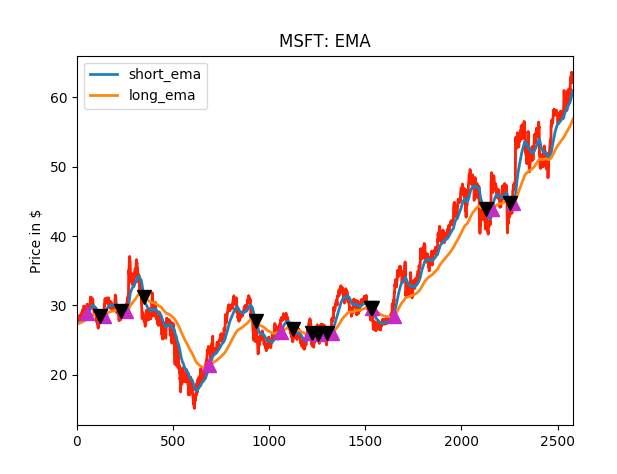
\includegraphics[width=90mm]{EMA_MSFT.png}
\caption{Dual Moving Average Strategy with Exponential effects applied to MSFT \label{overflow}}
\label{EMAfigure}
\end{figure}

\subsection{Bollinger Bands}

Bollinger Bands were introduced by John Bollinger in the 1980s\cite{Liu2006}. They provide a relative definition for high and low stock prices. This strategy uses 3 bands, with the 2 outer bands derived from a standard deviation of the moving average. Bollinger bands are great measures of market conditions of a particular security. Just like the previously examined techniques, the method uses a simple moving average as its basis, but instead incorporates 3 different bands separated by standard deviation. Because of this use of standard deviation, which is determined by market volatility, Bollinger Bands adjust themselves to market conditions. Precisely, the bands are calculated as follows with M - Middle Band, U - Upper Band, L - Lower Band, STD(x) - standard deviation of period x: \[M = SMA(12), U = M + 2 * STD(12),  L = M - 2 * STD(12)\] When the market is more volatile the bands widen and when the market becomes less erratic, the bands move closer together \cite{Liu2006}. Unlike the previous techniques, this strategy uses market conditions to evaluate trading orders.

This strategy is implemented with these 3 bands as mentioned above. For our implementation, a 12 day window was chosen to test out the algorithm, as this has been proven to be the most effective \cite{Liu2006}. When the closing price drops below the lower band, this gives a buy signal, as once a lower band has been broken due to heavy selling, the stock price will revert back and head towards the middle band. The opposite is true for when the closing price breaks the upper band, as this is indicative of heavy buying. The closing price approaching the upper band gives a bearish signal while approaching the lower band gives a bullish signal.  This strategy is showing in Figure~\ref{BBANDSfigure}. This measure can generate multiple buy or sell signals in a row. Looking at the first 100 days of the strategy, 5 straight sell signals are generated. The following 100 days subsequently generate 4 straight buy signals. This trend is indicative of the market giving only bearish indicators followed by a period of only bullish indicators stemming from the use of standard deviation in the measure.

\begin{figure}[h]
\centering
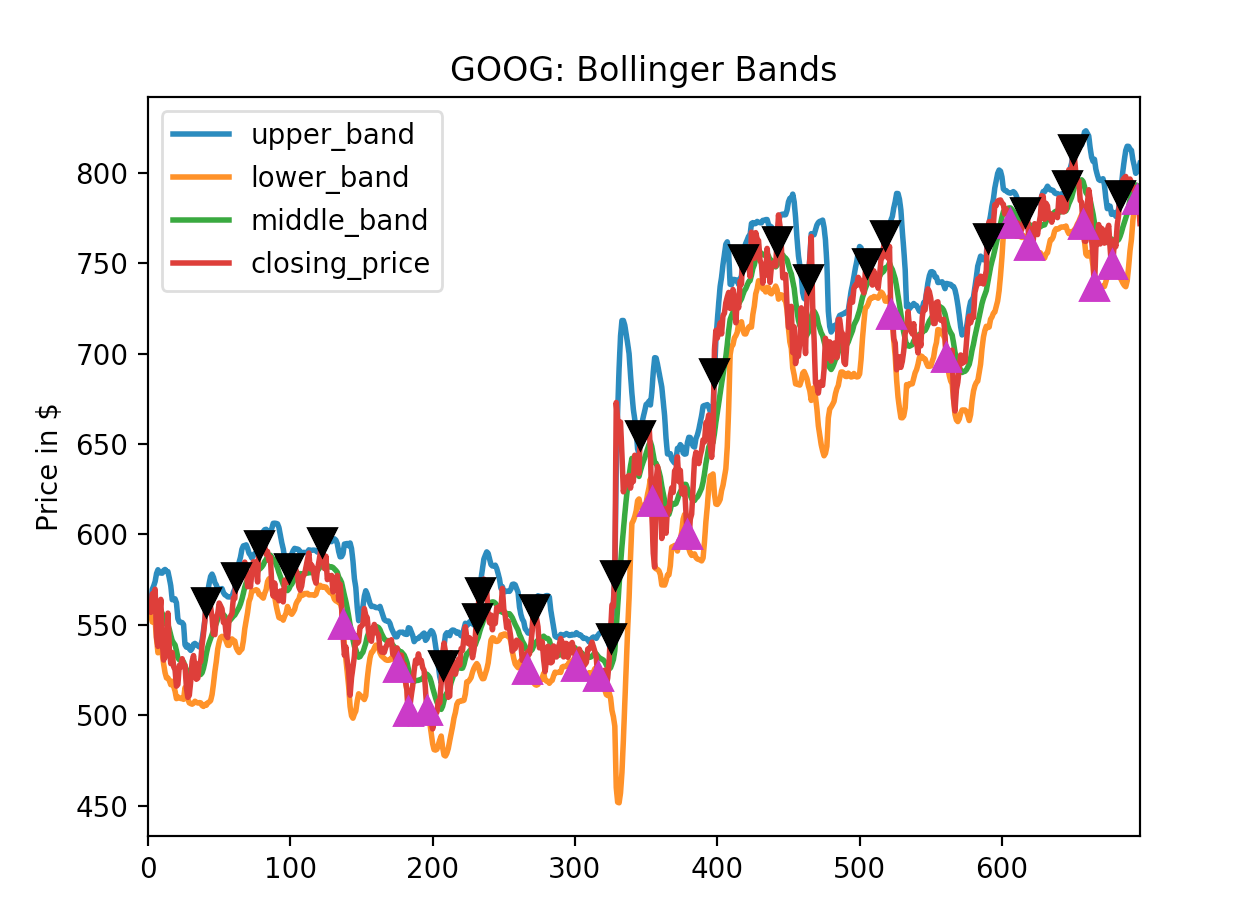
\includegraphics[width=90mm]{Goog_Bbands.png}
\caption{Bollinger Bands strategy applied to GOOG  \label{overflow}}
\label{BBANDSfigure}
\end{figure}

\subsection{RSI - Relative Strength Index}

Relative Strength Index (RSI) is a momentum indicator that measures the magnitudes of price changes to analyze overbought or oversold stocks. It demonstrates a particular security's recent performance over a relatively short window compared to the mean. This indicator is widely used today in algorithmic trading. The measure is a value between 0 and 100 at a specific date. The equation for RSI is as follows with $RS$ defined as average gain of up periods divided by the average gain of down periods over a specified window $x$ \cite{Chong2014}: \[RSI = 100.0 - (100.0 / (1.0 + RS(x))\] Therefore, a large RSI value is indicative of stocks that have had recent larger gains compared to losses while a low RSI value is indicative of stocks with poor recent performance compared to the mean.

This strategy takes advantage of mean reversion. Our implementation uses a very simple method. Sell signals are generated when the RSI is over 70 and buy signals are generated when the RSI is under 30 \cite{Chong2014}. This is very logical, as expected gains are the largest when a stock has performed poorly recently and is expected to revert back to the mean. This strategy also uses a 14 day window, which is standard across the industry. Figure~\ref{RSIfigure} shows this strategy when run on AAL. The second subfigure generates the buy and sell signals, as it shows the RSI of the stock throughout the period tested. These signals generated from the second subfigure are then plotted on the first subfigure over the stock price. Clearly, this strategy generates a large quantity of trading signals over the period.

\begin{figure}[h]
\centering

\begin{subfigure}[t]{0.45\textwidth}
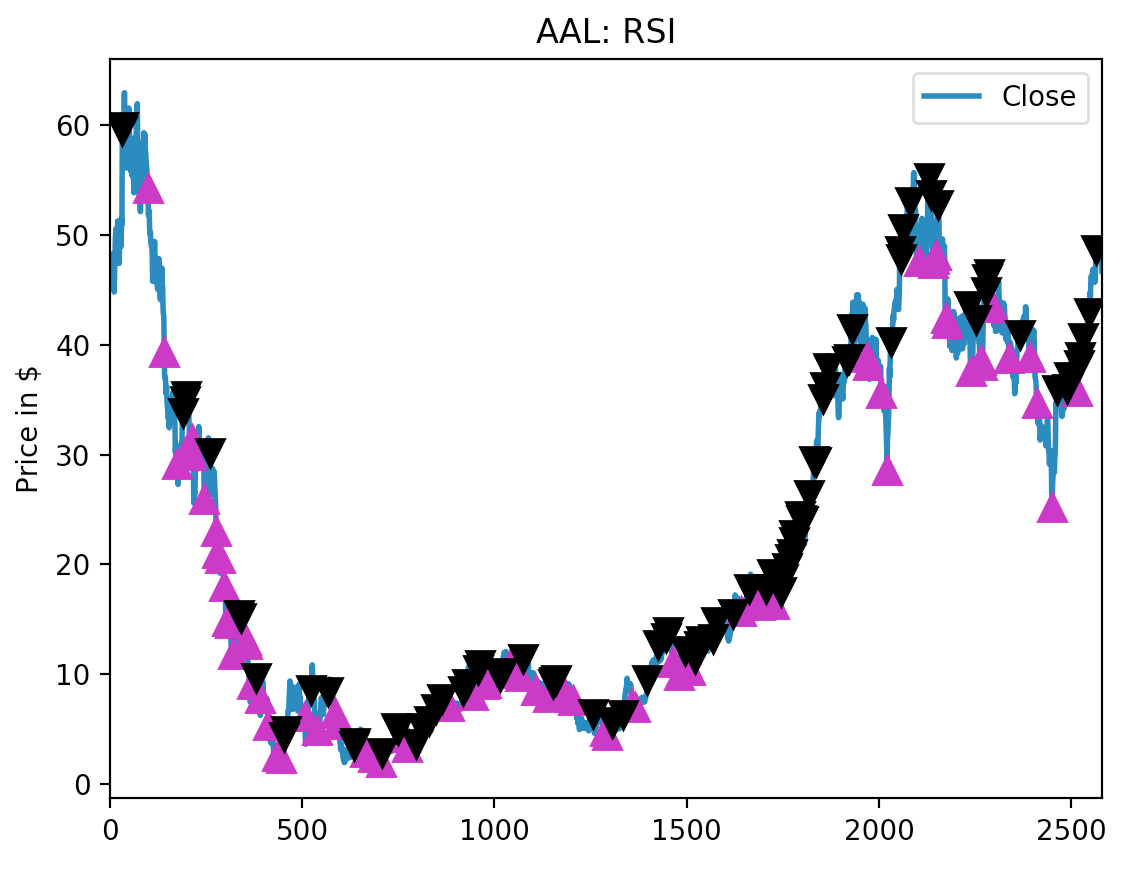
\includegraphics[width=\textwidth]{AAL_RSI_signals.png}
\caption{RSI Strategy \label{overflow}}
\end{subfigure}
\begin{subfigure}[t]{0.45\textwidth}
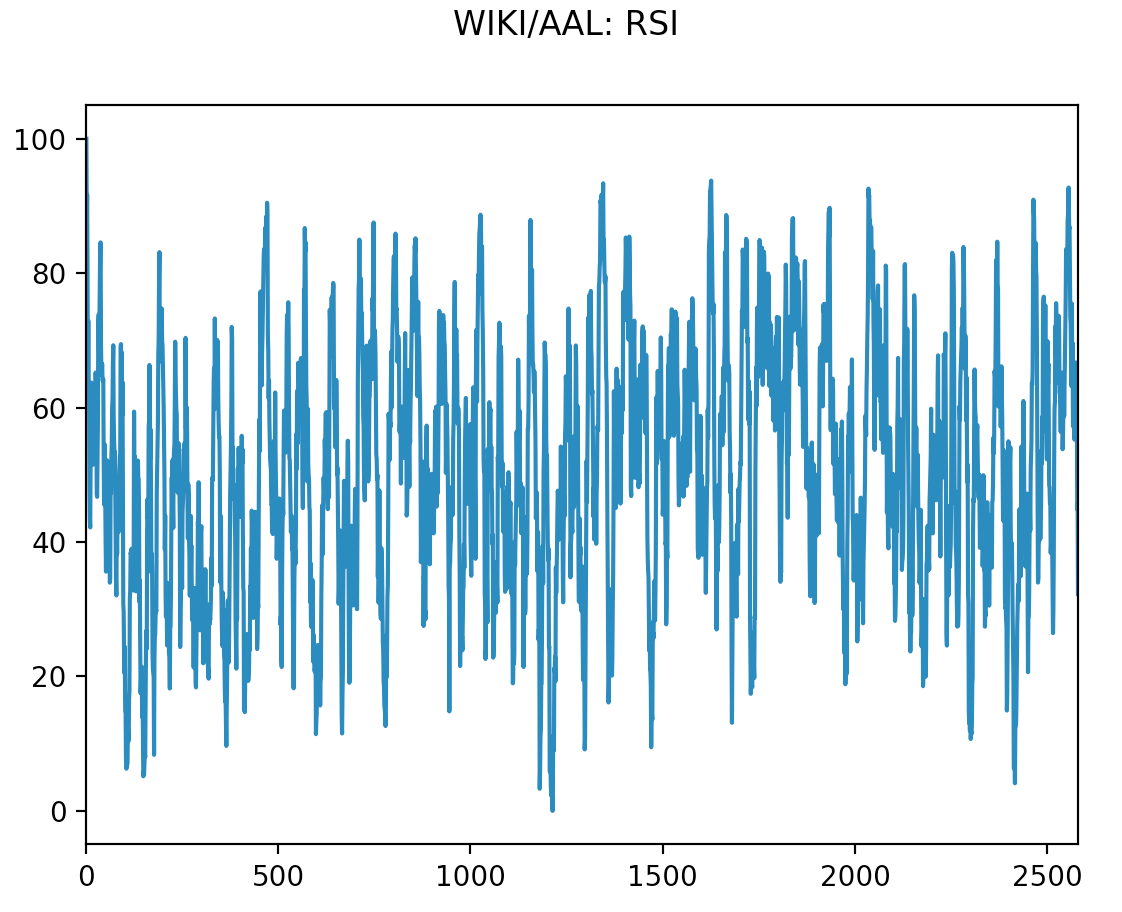
\includegraphics[width=\textwidth]{AAL_RSI.png}
\caption{ RSI of AAL \label{overflow}}
\end{subfigure}

\caption{RSI strategy applied to AAL  \label{overflow}}
\label{RSIfigure}
\end{figure}

\subsection{Combining Momentum Indicators - RSI and Moving Average Convergence-Divergence (MACD)}

MACD uses two moving averages to identify trend changes while RSI performs exactly as stated in the above section. The MACD is constructed by subtracting two different sized exponential moving averages from each other. The equation for MACD is as follows and uses $EMA(x)$, with $x$ representing the period in minutes \cite{Chong2014}: \[ MACD = EMA(12) - EMA(16)\] The MACD is then plotted against a signal line, which is defined as S and is the EMA of the 9 minute MACD: \[ S = EMA(MACD(9)) \] Buy and sell signals are then generated by the ``golden cross" method. Specifically, this is when the MACD crosses the signal line from below - signaling a momentum swing and a bullish buy signal. A sell signal is the reverse - when the MACD crosses the signal live from above. Figure~\ref{RSIMACDfigure}a shows the MACD strategy applied to AAPL. This strategy behaves the exact same way as both Figure~\ref{EMAfigure} and Figure~\ref{SMAfigure}.

Unlike the previously mentioned strategies, this one combines indicators to generate more robust trading signals. Because there are two different measures working at the same time, buy signals are generated by both the RSI and MACD measures giving bullish signals within 3 minutes of each other. Sell signals are generated by either one of the measures producing a sell. Under this strategy, buy signals are very rarely generated while either strategy generating a sell denotes all shares to be sold. Because of the selectivity of buy signals, we can expect this technique to be very profitable. This strategy is most effective when run over intra-day data because of the relative infrequency of buy signals as demonstrated in Figure~\ref{RSIMACDfigure}b. Throughout an entire day, only 2 buy signals were generated. 

\begin{figure}[h]
\centering

\begin{subfigure}[t]{0.45\textwidth}
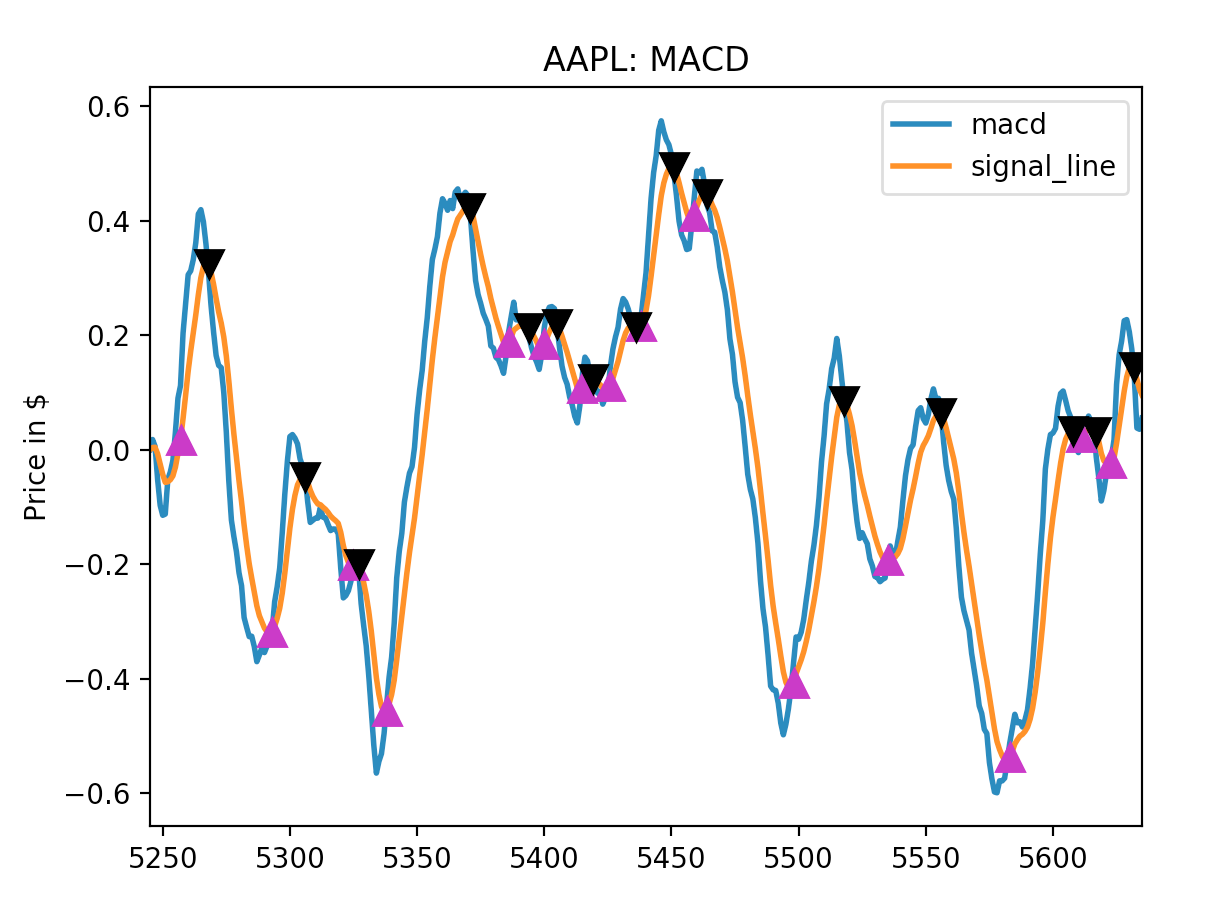
\includegraphics[width=\textwidth]{AAPL_MACD.png}
\caption{MACD Strategy \label{overflow}}
\end{subfigure}
\begin{subfigure}[t]{0.45\textwidth}
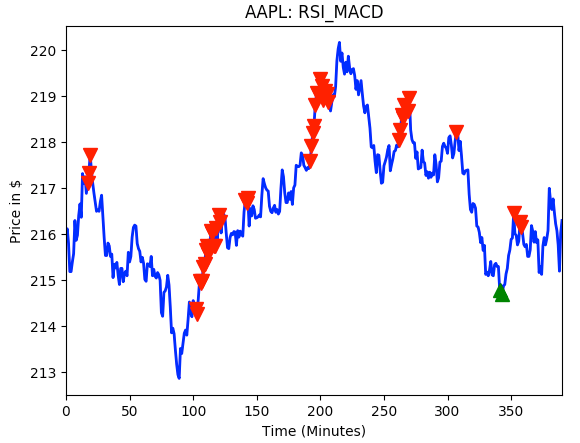
\includegraphics[width=\textwidth]{AAPL_RSIxMACD.png}
\caption{RSI and MACD strategy buy and sell signals \label{overflow}}
\end{subfigure}

\caption{RSI and MACD combination strategy applied to AAPL  \label{overflow}}
\label{RSIMACDfigure}
\end{figure}

\section{Pairs Trading - Arbitrage and Mean Reversion}

Pairs trading is an algorithmic trading strategy that chooses two economically linked stocks and profits off the divergence in spread of prices. Pairs trading uses statistical arbitrage, which is attempted profit from pricing inefficiencies identified through mathematical models. The most basic assumption is that prices will move towards their historical average, which pairs trading takes advantage of and is also known as mean reversion.  However, unlike other instances of mean-reversion, this strategy has a distinct advantage of always being hedged against market movements. 

Pairs trading is motivated by statistical arbitrage and mean reversion\cite{Fu2009}. When given two stocks that are linked economically (i.e. Pepsi and Coca-Cola), we expect the spread to remain relatively constant over time. However, there might be divergence in the spread between these two pairs cause by factors such as supply/demand changes or changes in volume in a particular stock.  Another problem with this is finding stocks that are closely related. Because we need to have stocks that behave similarly, we use cointegration to identify pairs of similarly behaving stocks. 

Cointegration is a stationary measure that highlights horizontal trends \cite{Gatev2006}. Unlike correlation, which only tracks similarly moving magnitudes over time, it instead tells how the difference between two regression lines changes over time. The implementation uses the python extension statsmodels to generate the p-value for cointegration. It is absolutely key to have related stocks, as this strategy takes advantage of mean reversion, or in other words, stocks reverting back to their original mean in relation to other similarly behaving ones. Now this is quite difficult, as it is very difficult to find stocks that are behave very similarly. After running comparisons of cointegration, certain tech stocks such as INTC and MFST were found to behave similarly.  

To generate trading signals, a Zscore is generated from the ratio of prices R(i) = ClosingPriceStockX/ClosingPriceStockY on a particular day $i$, the overall mean of ratio of prices M = AVG(R), and the standard deviation of the price ratio STD = STD(R): \[ Z = (R(i) - M)/STD\] The Zscore is a measure of how far away the current ratio of prices is away from its mean. Figure~\ref{PAIRSfigure}b shows the Zscore of both INTC and MSFT. Because of mean reversion, we can use this as a good indicator for buy and sell signals. A buy signal is generated when the zscore drops below -1, as we expect the zscore to return to its mean of 0. A sell signal is generated when the zscore goes above 1, as the stock is currently overvalued because we expect the stock to return to its mean of 0\cite{Fu2009}. These thresholds are shown in Figure~\ref{PAIRSfigure}b. In context of the pair of stocks, on buy signals the first stock in the pair is bought while the second is sold or shorted. The reverse is true on sell signals. Figure~\ref{PAIRSfigure} shows this strategy applied to INTC and MSFT. The red triangles represent sell signals while the green triangles show buy signals. Each time a buy signal is generated at a particular day the other stock has a matching sell signal and vice versa.

\begin{figure}[h]
\centering
\begin{subfigure}[t]{0.45\textwidth}
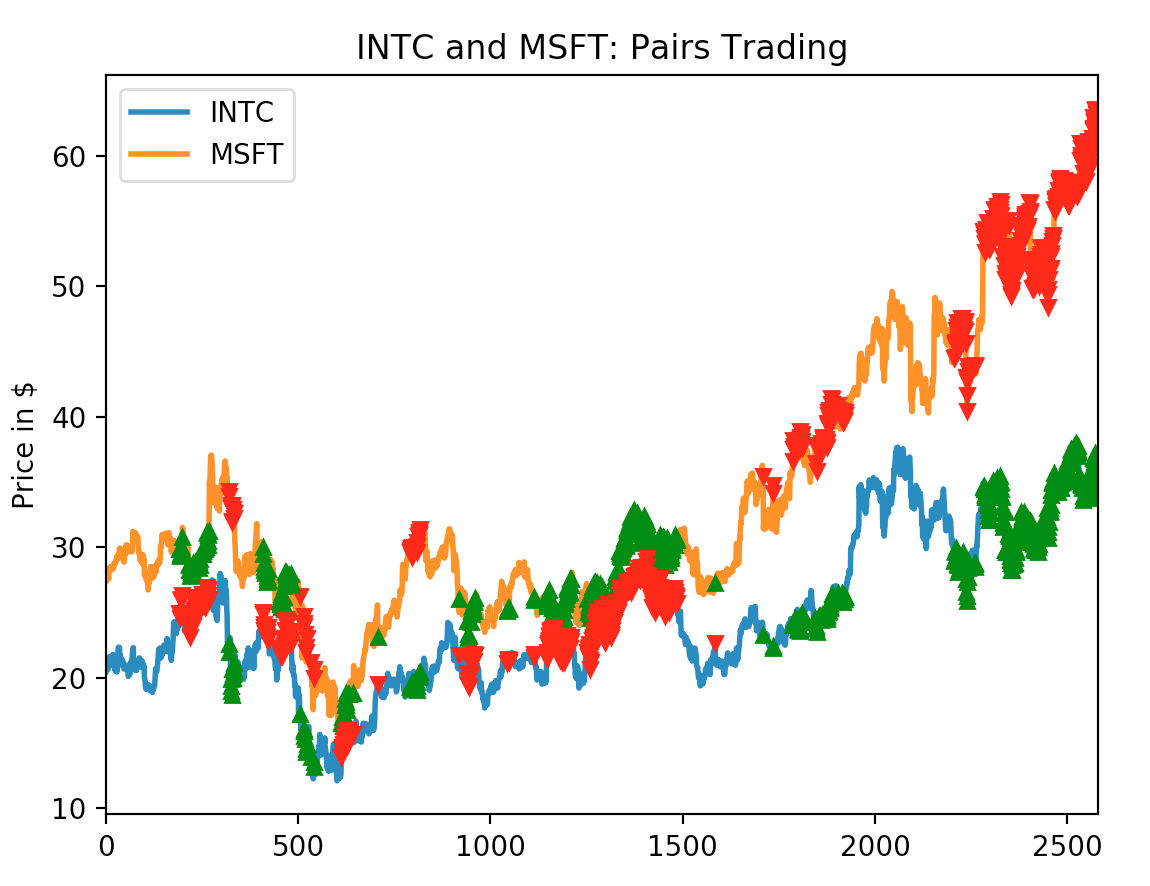
\includegraphics[width=\textwidth]{Intc_msft_signals.png}
\caption{Pairs Trading Strategy  \label{overflow}}
\end{subfigure}
\begin{subfigure}[t]{0.45\textwidth}
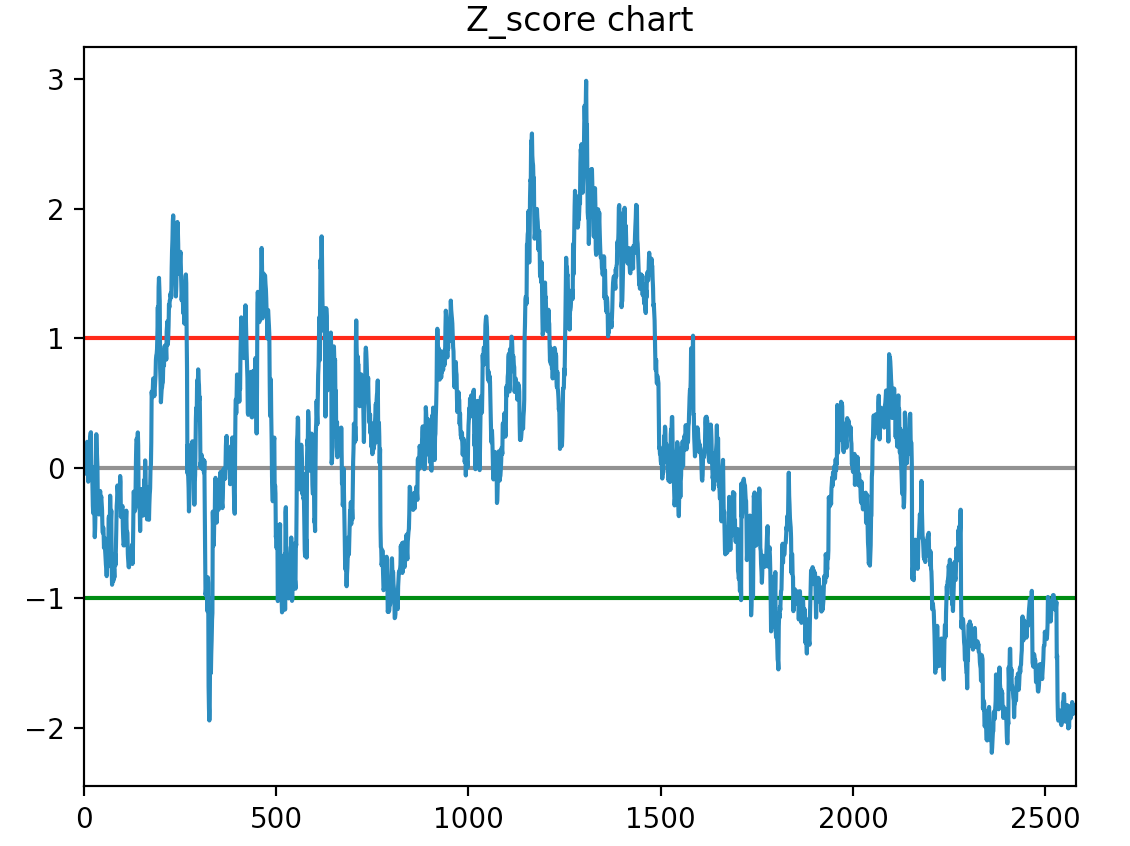
\includegraphics[width=\textwidth]{zscore.png}
\caption{Zscore of INTC and  MSFT \label{overflow}}
\end{subfigure}

\caption{Pairs Trading strategy applied to INTC and MSFT  \label{overflow}}
\label{PAIRSfigure}
\end{figure}

\end{document}
